\protect \section *{\nameref *{Electrostatics}}
\begin{Solution}{1.{1}}
	$E = \frac{4E_1E_2}{(\sqrt{E_1} + \sqrt{E_2})^2}$.
\end{Solution}
\begin{Solution}{1.{4}}
	$E = \frac{2\lambda}{r}.$
\end{Solution}
\begin{Solution}{1.{5}}
	$E_z = 2\pi\sigma \left( 1 - \frac{z}{\sqrt{R^2 + z^2}}\right)$
\end{Solution}
\begin{Solution}{1.{6}}
	$E_z = 2\pi\sigma$.
\end{Solution}
\begin{Solution}{1.{7}}
	$E_z = \pi\sigma$.
\end{Solution}
\begin{Solution}{1.{8}}
	$E=2\sqrt{2}\pi\sigma$
\end{Solution}
\begin{Solution}{1.{9}}
	\begin{enumerate*}[label=\alph*)]
		\item $E = \frac{\pi\lambda_0}{R}$;
		\item $E = \frac{\pi\lambda_0R^2}{\left( z^2 + R^2\right)^{\nfrac{3}{2}}}$.
	\end{enumerate*}
\end{Solution}
\begin{Solution}{1.{10}}
	$\Efield = 2\pi\sigma\frac{\vect{r}}{r} - 2d\sigma\frac{\vect{r}}{r^2}$, де $\vect{r}$~--- радіус-вектор проведений від осі симетрії щілини в точку спостереження.
\end{Solution}
\begin{Solution}{1.{11}}
	$\Efield = \frac43 \pi R \vect{a}$
\end{Solution}
\begin{Solution}{1.{12}}
	$E_z = \pi\sigma$.
\end{Solution}
\begin{Solution}{1.{13}}
	$E_z = \frac{2\pi\sigma z}{\sqrt{R^2 + z^2}}$
\end{Solution}
\begin{Solution}{1.{14}}
	$E_z = 2\pi\sigma$.
\end{Solution}
\begin{Solution}{1.{15}}
	$\Efield =-\frac{\pi r^2 \sigma}{R^3}\vect{r}$, де $\vect{r}$~--- радіус-вектор з початком у центрі вирізаного отвору і кінцем у центрі сфери.
\end{Solution}
\begin{Solution}{1.{16}}
	$\Phi = \pi l \lambda$
\end{Solution}
\begin{Solution}{1.{17}}
	$\Phi = 2\pi\lambda R$.
\end{Solution}
\begin{Solution}{1.{18}}
	Потік через куб $\Phi = \frac{\pi}{2}q$. Потік через грані, що сходяться у вершині, в якій розташований заряд $\Phi_1 = \Phi_2 =\Phi_3 = 0$, потік через інші грані $\Phi_4 = \Phi_5 =\Phi_6 = \frac{\pi}{6}q$.
\end{Solution}
\begin{Solution}{1.{19}}
	$\Phi = 2\pi q\left( 1 - \frac{l}{\sqrt{R^2 + l^2}}\right) $.
\end{Solution}
\begin{Solution}{1.{21}}
	$\Efield =
		\begin{cases}
			2\pi\rho r\\
			\frac{2\pi\rho R^2}{r}.
		\end{cases}
	$
\end{Solution}
\begin{Solution}{1.{22}}
	$E =
		\begin{cases}
			\rho\frac{4\pi\rho}{3}r\\
			\rho\frac{4\pi\rho R^3}{3 r^2}.
		\end{cases}
	$
\end{Solution}
\begin{Solution}{1.{23}}
	$\Efield = 2\pi\rho \vect{l}$, де $\vect{l}$~--- вектор, проведений від центру циліндра до центру порожнини.
\end{Solution}
\begin{Solution}{1.{24}}
	$\Efield = \frac{4\pi}{3}\rho \vect{l}$, де $\vect{l}$~--- вектор, проведений від центру кулі до центру порожнини.
\end{Solution}
\begin{Solution}{1.{25}}
	$q = 2\pi a R^2$
\end{Solution}
\begin{Solution}{1.{26}}
	$\Efield = \frac{e\vect{r}}{r^3} \left[ 1 + \frac{2r}{a} \left( 1 + \frac{r}{a} \right) \right]\exp{\left( -\frac{2r}{a}\right) }$. При $r\ll a$, $\Efield = \frac{e\vect{r}}{r^3}$, при $r \gg a$, $\Efield = \frac{2e\vect{r}}{a^2r}\exp{\left( -\frac{2r}{a}\right) }.$
\end{Solution}
\begin{Solution}{1.{28}}
	$E_z = \frac{\pi qR}{2z^3}$
\end{Solution}
\begin{Solution}{1.{29}}
	$V = \frac{E_1}{E_2}2\pi l^3$.
\end{Solution}
\begin{Solution}{1.{30}}
	\begin{enumerate*}[label=\alph*)]
		\item $F = \frac{3 p_1 p_2}{d^4}$, диполі відштовхуються,
		\item $F = \frac{3 p_1 p_2}{d^4}$, диполі притягуються,
		\item $F = \frac{6 p_1 p_2}{d^4}$, диполі притягуються,
		\item $F = \frac{6 p_1 p_2}{d^4}$, диполі відштовхуються.
	\end{enumerate*}
\end{Solution}
\begin{Solution}{1.{31}}
	Вказівка: Сила, що діє на диполь в неоднорідному магнітному полі визначається за формулою $\vect{F} = (\vect{p}\cdot\nabla)\Efield$, а момент сили $\vect{M} = \left[ \vect{p}\times\Efield\right]  + \left[ \vect{r}\times\vect{F}\right] $.

	\begin{enumerate*}[label=\alph*)]
		\item $\vect{F} = 0$, $\vect{M} = \frac{2\lambda}{r^2} \left[ \vect{p}\times\vect{r}\right] $,
		\item $\vect{F} = \frac{2\lambda \vect{p}}{r^2}$, $\vect{M} = 0$,
		\item $\vect{F} = \frac{2\lambda \vect{p}}{r^2}$, $\vect{M} = 0$.
	\end{enumerate*}
\end{Solution}
\begin{Solution}{1.{33}}
	$M_1 = -\frac{p^2}{r^3}$, $M_2 = -\frac{2p^2}{r^3}$. Обертовий момент, що діє на систему дорівнює нулю.
\end{Solution}
\begin{Solution}{1.{34}}
	$\vect{p} = \Efield_0 R^3$,
	$\sigma = \frac{3}{4\pi} \frac{\left( \Efield_0\cdot\vect{r}\right) }{r}$,
	$Q = \frac34 E_0 R^2$
\end{Solution}
\begin{Solution}{1.{35}}
	\begin{enumerate*}[label=\alph*)]
		\item $F = \frac{6\Efield_0^2R^6}{l^4}$, кулі притягуються,
		\item $F = \frac{3\Efield_0^2R^6}{l^4}$, кулі відштовхуються.
	\end{enumerate*}
\end{Solution}
\begin{Solution}{1.{38}}
	$\frac{\phi_1}{\phi_2} =\sqrt\eta$.
\end{Solution}
\begin{Solution}{1.{43}}
	$\phi = -\Efield\cdot\vect{r}$, де $\vect{r}$~-- радіус вектор довільної точки поля.
\end{Solution}
\begin{Solution}{1.{44}}
	$\phi = \frac{q}{r} + \frac{q}{4r}\left(\frac{R}{r} \right)^2(1-3\cos^2\theta) $
\end{Solution}
\begin{Solution}{1.{45}}
	$\Delta\phi = \frac{2q}{R}\left(1 - \frac{1}{\sqrt{1 + \left(\frac{a}{R} \right)^2}}\right)$
\end{Solution}
\begin{Solution}{1.{46}}
	$\phi = 2\pi\sigma  \left( \sqrt{R^2 + z^2} - z \right) $.
\end{Solution}
\begin{Solution}{1.{48}}
	$\phi = -\frac43\pi R (\vect{a}\cdot\vect{r})$.
\end{Solution}
\begin{Solution}{1.{56}}
	Так. Відповідь обґрунтовується за допомогою теореми Гауса та теореми про циркуляцію.
\end{Solution}
\begin{Solution}{1.{60}}
	\begin{enumerate}[label=\alph*)]
		\item $\phi =
		      \begin{cases}
			  \frac{\sigma \pi R^2}{R}, \,    & r < R, \\
			  \frac{\sigma \pi R^2}{r}, \, & r > R
			  \end{cases}
			  $,
		\item $\phi =
			      \begin{cases}
				      \frac23 \pi \rho (3R^2 - r^2), \,    & r < R, \\
				      \frac{4\pi R^3}{3}\frac{\rho}{r}, \, & r > R
			      \end{cases}
		      $,
		\item $\phi =
			      \begin{cases}
				      \lambda \left(1- \frac{r^2}{R^2} \right) ,\, & r < R, \\
				      -2\lambda\ln\frac{r}{R}, \,                  & r > R
			      \end{cases}
		      $,
		\item $\phi =
			      \begin{cases}
				      -2\pi\rho z^2, \,                      & \left| z\right| < a,  \\
				      2\pi\rho a (a - 2\left| z\right| ), \, & \left| z\right| \ge a
			      \end{cases}
		      $
	\end{enumerate}
\end{Solution}
\begin{Solution}{1.{61}}
		\[
		\phi = \begin{cases}
				0, \quad -\infty< x < -a \\
				2\pi\rho_0 (x+a)^2, \quad -a \le x \le 0, \\
				-2\pi\rho_0 (x-a)^2 + 4\pi\rho_0a^2, \quad 0 \le x \le a, \\
				4\pi\rho_0a^2, \quad a < x < \infty,
				\end{cases}
		\]
		\[
		E = \begin{cases}
				0, \quad -\infty< x < -a \\
				-4\pi\rho_0 (x+a), \quad -a \le x \le 0, \\
				4\pi\rho_0 (x-a), \quad 0 \le x \le a, \\
				0, \quad a < x < \infty,
				\end{cases}
		\]
	
\end{Solution}
\begin{Solution}{1.{62}}
	$
		\phi(r) =
		\begin{cases}
			4\pi a\ln\frac{R_2}{R_1},                                                  & r \le R_1         \\
			4\pi a \left[ \left( 1- \frac{R_1}{r}\right)  + \ln\frac{R_2}{r} \right] , & R_1 \le r \le R_2 \\
			4\pi a \frac{R_2 - R_1}{r},                                                & r \ge R_2
		\end{cases}
	$
\end{Solution}
\begin{Solution}{1.{63}}
	$E = \frac{\pi\rho_0}{a}(e^{aR} - 1)$.
\end{Solution}
\begin{Solution}{1.{64}}
	$\rho = \frac{3a}{2\pi}$.
\end{Solution}
\begin{Solution}{1.{65}}
	Розподіл зарядів знайдемо з рівняння Пуассона:
	\[
		\Delta\phi = -4\pi\rho.
	\]
	Розпишемо
	\begin{multline*}
		\Delta\phi = \divg\vect{\nabla}\phi = \divg\vect{\nabla}\left( \frac{q}{r}e^{-\frac{r}{a}}\right)  = \\
		= \divg\left( \frac{q}{r}  \vect{\nabla}e^{-\frac{r}{a}} + e^{-\frac{r}{a}}\vect{\nabla}\frac{q}{r}\right) = \\
		= \vect{\nabla}\left( \frac{q}{r}\right) \vect{\nabla}e^{-\frac{r}{a}} + \frac{q}{r}\Delta e^{-\frac{r}{a}} +
		\vect{\nabla}e^{-\frac{r}{a}} \vect{\nabla}\left( \frac{q}{r}\right)  + e^{-\frac{r}{a}}\Delta\left( \frac{q}{r}\right) = \\
		= e^{-\frac{r}{a}}\Delta\left( \frac{q}{r}\right) + 2 \vect{\nabla}\left( \frac{q}{r}\right)\cdot \vect{\nabla}e^{-\frac{r}{a}} + \frac{q}{r}\Delta e^{-\frac{r}{a}} =\\
		= -4\pi q\delta(r)	+ \frac{q}{a^2}\frac{e^{-\frac{r}{a}}}{r}
	\end{multline*}
	Співставляючи останній вираз з рівнянням Пуассона, знайдемо розподіл заряду:
	\[
		\rho = q\delta(r) - \frac{q}{4\pi a^2} \frac{e^{-\frac{r}{a}}}{r},
	\]
	звідки видно, що екранований кулонівський потенціал створюється точковим зарядом, навколо якого розподілена <<хмара>> електричного заряду. Такий характер розподілу зустрічається, наприклад, в електролітах, або плазмі.
\end{Solution}
\begin{Solution}{1.{66}}
	$\rho = \frac{eb^2}{4\pi r}e^{-br}$ при $r \neq 0$. $Q = 0$.
\end{Solution}
\begin{Solution}{1.{67}}
	$\rho_{\mathrm{in}} = \rho_0\left( 1 - \frac{r}{R}\right)$, при $r <R$, $\rho_{\mathrm{out}} = 0$, при $r > R$.
\end{Solution}
\begin{Solution}{1.{68}}
	$\left. \sigma\right|_{x=0} = 0$, $\left. \sigma\right|_{x=d} = -\frac{1}{3\pi}kd^{\frac13}$ , $\rho = -\frac{k}{9\pi} x^{-\frac{2}{3}}$.
\end{Solution}
\begin{Solution}{1.{74}}
		$\phi = \frac{q}{l} + \frac{Q}{R}.$
	
\end{Solution}
\begin{Solution}{1.{75}}
		$\phi = \frac{q}{R} + \frac{Q}{R}.$
	
\end{Solution}
\begin{Solution}{1.{76}}
	$\phi_1 = \phi_2 = \frac{Q_1 + Q_2}{R_1 + R_2}$, $q_1 = (Q_1 + Q_2) \frac{R_1}{R_1 + R_2}$, $q_2 = (Q_1 + Q_2) \frac{R_2}{R_1 + R_2}$,
\end{Solution}
\begin{Solution}{1.{77}}
	$q_1 = -Q\frac{R_2-R}{R_2-R_1}\frac{R_1}{R}$, $q_2 = -Q\frac{R-R_1}{R_2-R_1}\frac{R_2}{R}$
\end{Solution}
\begin{Solution}{1.{78}}
	$
		\phi(r) =
		\begin{cases}
			\frac{q_1}{R_1} + \frac{q_2}{R_2}, & r \le R_1         \\
			\frac{q_2}{R_2} + \frac{q_1}{r} ,  & R_1 \le r \le R_2 \\
			\frac{q_1 + q_2}{r} ,              & r \ge R_2
		\end{cases}
	$
\end{Solution}
\begin{Solution}{1.{79}}
	$\phi = q\left( \frac{1}{r} - \frac{1}{R_1} + \frac{1}{R_2}\right) $
\end{Solution}
\begin{Solution}{1.{80}}
	$q=Q\left( \frac{R_2}{R_3} - 1\right) $
\end{Solution}
\begin{Solution}{1.{81}}
	$q_1 = - Q\frac{R_3 - R_2}{R_3 - R_1}\cdot \frac{R_1}{R_2}$, $q_2= -q_1$,
	$
		E(r) =
		\begin{cases}
			0,                 & r < R_1       \\
			\frac{q_1}{r^2},   & R_1 < r < R_2 \\
			\frac{Q+q_1}{r^2}, & R_2 < r < R_3 \\
			\frac{Q}{r^2},     & r > R_3
		\end{cases}
	$,

	$
		\phi(r)~=~%
		\begin{cases}
			\frac{q_1}{R_1} + \frac{Q}{R_2} - \frac{q_1}{R_3}, & r < R_1       \\
			\frac{q_1}{r} + \frac{Q}{R_2} - \frac{q_1}{R_3},   & R_1 < r < R_2 \\
			\frac{Q+q_1}{r},                                   & R_2 < r < R_3 \\
			\frac{Q}{r},                                       & r > R_3
		\end{cases}
	$.
\end{Solution}
\begin{Solution}{1.{82}}
	$q_1 = -Q\frac{R_1(R_3 - R_2)}{R_2(R_3 - R_1)}$, $q_2 = Q\frac{R_3(R_2 - R_1)}{R_2(R_3 - R_1)}$.
\end{Solution}
\begin{Solution}{1.{83}}
	$\Delta\phi = \frac{2\pi Q}{S} (d_2 - d_1)$.
\end{Solution}
\begin{Solution}{1.{85}}
	$Q_{L} = \frac{Q_2 - Q_1}{2}$, $Q_{R} = -Q_{L}$.
\end{Solution}
\begin{Solution}{1.{86}}
	$Q_1 = -\frac{Q}{2}\frac{d_2 - d_1}{d_2 + d_1}$, $Q_2 = - Q_1$.
\end{Solution}
\begin{Solution}{1.{87}}
	$Q_2 = -\frac{Q}{2}$, $Q_3 = \frac{Q}{2}$.
\end{Solution}
\begin{Solution}{1.{88}}
	$Q_2 = -\frac{q_0}{2} -\frac{\EMF S}{4\pi d}$, $Q_3 = \frac{q_0}{2} + \frac{\EMF S}{4\pi d}$.
\end{Solution}
\begin{Solution}{1.{89}}
	$Q_1 = -\frac{2\EMF S + 4\pi Q(d_2 - d_1)}{8\pi(d_1 + d_2)}$, $Q_3 = -Q_1$.
\end{Solution}
\begin{Solution}{1.{90}}
	\begin{enumerate*}[label=\alph*)]
	\item  $q'$,
	\item  $-q$.
	\end{enumerate*}
\end{Solution}
\begin{Solution}{1.{91}}
		$p = \frac{R^3}{l^2} q$.
	
\end{Solution}
\begin{Solution}{1.{92}}
	$ F =  \frac{qq_0}{b^2} + \frac{q^2 R}{b^3} - \frac{q^2 Rb}{(b^2 - R^2)^2}$.
\end{Solution}
\begin{Solution}{1.{93}}
	$\sigma_a = -\frac{q_a}{4\pi a^2}$, $\sigma_b = -\frac{q_a}{4\pi b^2}$, $\sigma_R = \frac{q_a + q_b}{4\pi R^2}$.
\end{Solution}
\begin{Solution}{1.{94}}
	\begin{enumerate*}[label=\alph*)]
		\item $F = \frac{q^2Rb}{(b^2-R^2)^2} $,
		\item $F = q^2R\left( \frac{b}{(b^2-R^2)^2} - \frac{1}{b^3}\right)$,
		\item $F = \frac{qQ}{b^2} - \frac{q^2R^3(2b^2 - R^2)}{b^3(b^2 - R^2)^2}$.
	\end{enumerate*}
\end{Solution}
\begin{Solution}{1.{95}}
	$F = -\frac{qRa}{(a^2 - R^2)^2}$. Якщо кулю буде незаземленою, результат не зміниться. Сила взаємодії не залежить від заряду кулі.
\end{Solution}
\begin{Solution}{1.{96}}
	$\sigma_{in} = \frac{q}{18\pi r^2}$, $\sigma_{out} = - \frac{q}{4\pi r^2}$. Після заземлення $\sigma_{in} = \frac{q}{18\pi r^2}$, $\sigma_{out} = 0$.
\end{Solution}
\begin{Solution}{1.{98}}
	$F = \frac{2\lambda^2}{R\left( 1 - \nfrac{r^2}{R^2}\right) }$.
\end{Solution}
\begin{Solution}{1.{99}}
	$F = \frac{3p^2R^3}{b^7}$, взаємодія~--- притягування.
\end{Solution}
\begin{Solution}{1.{100}}
	Згідно методу зображень, металева куля створює заряд-зображення $dq'$ елемента поверхні диска, на якому міститься заряд $dq = \sigma dS$, де $\sigma = \frac{q}{\pi R^2}$. Величину заряду-зображення (заряд кулі) можна знайти як:
	\[
		q' = - \int\frac{R}{r}\sigma dS.
	\]

	Для інтегрування, зручно скористатись елементом тілесного кута, під яким видно елемент диска з центру сфери:
	\[
		d\Omega = \frac{dS\cos\theta}{r^2}.
	\]

	Отже
	\[
		q' = - 2\pi R^2\int\limits_{0}^{\nfrac{\pi}{4}} \frac{\sin\theta}{\cos^2\theta}d\theta = -2(\sqrt2 - 1)q.
	\]
\end{Solution}
\begin{Solution}{1.{101}}
	$\phi = \frac{Q}{r_1} + \frac{q}{r_2} + \frac{Q+q}{R}$.
\end{Solution}
\begin{Solution}{1.{104}}
		\begin{enumerate*}[label=\alph*)]
			\item $\vect{E} = \pm 2\pi \vect{P}$,
			\item $\vect{E} = -2\pi \vect{P} \left(\frac{r}{l} \right)^2$,
			\item величину і напрямок поля на поверхні циліндра поблизу його центра приблизно дорівнює полю в його центрі.
		\end{enumerate*}
		$\vect{E}_A = 4\pi \vect{P}$, $\vect{P}$
	
\end{Solution}
\begin{Solution}{1.{105}}
		Поле зовні $\vect{E} = 2\pi\vect{P}\frac{d}{R}$, поле в середині $\vect{E} = -2\pi\vect{P}\left( 2 - \frac{d}{R}\right) $.
		Індукція зовні та в середині $\vect{D} = 2\pi\vect{P}\frac{d}{R}$.
	
\end{Solution}
\begin{Solution}{1.{107}}
	\begin{enumerate*}[label=\alph*)]
		\item $\oint\limits_{S} \Efield d\vect{S} = \frac{\epsilon  -1}{\epsilon} \pi R^2 E_0 \cos\theta$,
		\item $\oint\limits_{\Gamma} \Dfield d\vect{r} = - \left( \epsilon -1\right)  l E_0 \sin\theta$.
	\end{enumerate*}
	
\end{Solution}
\begin{Solution}{1.{108}}
		$\epsilon_2 \tg\theta_1 = \epsilon_1 \tg\theta_2$, де $\theta_1$ та $\theta_2$~--- кути між нормаллю до поверхні та силовими лініями в діелектрику $1$ та $2$, відповідно.
	
\end{Solution}
\begin{Solution}{1.{109}}
	$\Efield = -4\pi \vect{P} \left( 1 - \frac{l}{\sqrt{4R^2 + l^2}}\right)$.
\end{Solution}
\begin{Solution}{1.{110}}
	$\Efield = -2\pi \vect{P} \frac{l}{\sqrt{4R^2 + l^2}}$.
\end{Solution}
\begin{Solution}{1.{111}}
	\[
	\Efield =
	\begin{cases}
	- \frac{4\pi}{3}\vect{P},                                                                                   & r \le R \\
	\frac{4\pi}{3}R^3\left( \frac{\vect{P}}{r^3} + \frac{3\left(\vect{P}\vect{r}\right)\vect{r} }{r^5}\right) , & r > R.
	\end{cases}
	\]
\end{Solution}
\begin{Solution}{1.{112}}
	$\lambda = 0$,
	$\Dfield = 0$ у всьому просторі,
	$\Efield = %
		\begin{cases}
			- 4\pi  a  \vect{r}, & \quad r < R \\
			0,                              & \quad r > R
		\end{cases}
	$.
\end{Solution}
\begin{Solution}{1.{113}}
		$E_1 = 4\pi P\frac{h}{d}$, $E_2  =4\pi P \left( 1 - \frac{h}{d}\right) $, $D_1 = D_2 = E_1$.
	
\end{Solution}
\begin{Solution}{1.{114}}
		Заряди на поверхні кулі, яка знаходиться у вакуумі $\sigma_1 = \frac{q}{2\pi R (\epsilon + 1)}$, на поверхні, що занурена в діелектрик~--- $\sigma_2 = \epsilon \frac{q}{2\pi R (\epsilon + 1)}$.
		%=========================================================
		\begin{center}
			%---------------------------------------------------------
			\begin{minipage}[t]{0.45\linewidth}\centering
				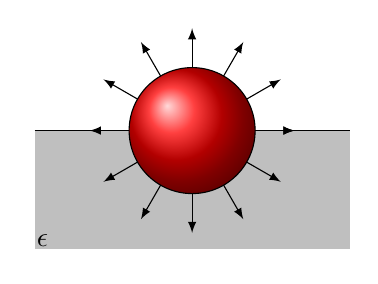
\begin{tikzpicture}
				\def\R{0.8}
				\fill[gray!50] (-2,-1.5) rectangle (2,0);
				\node at (-1.9,-1.4) {$\epsilon$};
				\draw[] (-2,0) -- (2,0);
				\coordinate (P) at (0,0);
				\foreach \i in {0,...,12} {\draw[-latex] (P) -- ({30*\i}:{\R+0.5});}
				\draw[ball color=red] (P) circle (\R);
				\end{tikzpicture}
				\captionof{figure}{Картина ліній вектора $\vect{E}$}
				\label{}
			\end{minipage}
			%---------------------------------------------------------
			\begin{minipage}[t]{0.45\linewidth}\centering
				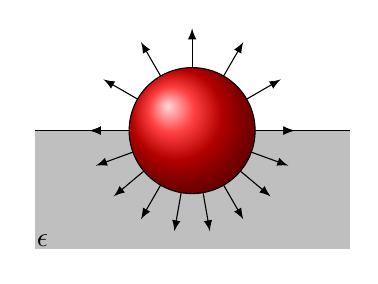
\begin{tikzpicture}
				\def\R{0.8}
				\fill[gray!50] (-2,-1.5) rectangle (2,0);
				\node at (-1.9,-1.4) {$\epsilon$};
				\draw[] (-2,0) -- (2,0);
				\coordinate (P) at (0,0);
				\foreach \i in {0,...,6} {\draw[-latex] (P) -- ({30*\i}:{\R+0.5});}
				\foreach \i in {9,...,18} {\draw[-latex] (P) -- ({20*\i}:{\R+0.5});}
				\draw[ball color=red] (P) circle (\R);
				\end{tikzpicture}
				\captionof{figure}{Картина ліній вектора $\vect{D}$}
			\end{minipage}
			%---------------------------------------------------------
		\end{center}
		%=========================================================
	
\end{Solution}
\begin{Solution}{1.{115}}
	$\phi = \frac{2}{\epsilon_1 + \epsilon_2} \frac{q}{r}$,
	$\Efield = \frac{2}{\epsilon_1 + \epsilon_2} \frac{q\vect{r}}{r^3}$,
	$\Dfield =
		\begin{cases}
			\frac{2\epsilon_1}{\epsilon_1 + \epsilon_2} \frac{q\vect{r}}{r^3}, & \text{в діелектрику 1} \\
			\frac{2\epsilon_2}{\epsilon_1 + \epsilon_2} \frac{q\vect{r}}{r^3}, & \text{в діелектрику 2}
		\end{cases}
	$
\end{Solution}
\begin{Solution}{1.{116}}
		У випадку паралельного заповнення до обкладок:
		\begin{enumerate*}[label=\alph*)]
			\item за постійної напруги
			$E_1 = \frac{2\epsilon}{\epsilon + 1} E_0$, $E_2 = \frac{2}{\epsilon + 1} E_0$, $D_1 = D_2 = \frac{2\epsilon}{\epsilon + 1} E_0$;
			\item за постійного заряду
			$E_1 = E_0$, $E_2 = \frac{E_0}{\epsilon}$, $D_1 = D_2 = E_0$.
		\end{enumerate*}
		У випадку перпендикулярно заповнення до обкладок:
		\begin{enumerate*}[label=\alph*)]
			\item за постійної напруги
			$E_1 = E_2 = E_0$, $D_1 = E_0$, $D_2 = \epsilon D_1$;
			\item за постійного заряду
			$E_1 = E_2 = \frac{2}{\epsilon + 1} E_0$, $D_1 = \frac{2}{\epsilon + 1} E_0$, $D_2 = \epsilon D_1$.
		\end{enumerate*}
	
\end{Solution}
\begin{Solution}{1.{117}}
	$\vect{p} = \frac{\epsilon - 1}{\epsilon + 2}R^3\Efield_0$,
	$
		\Efield =
		\begin{cases}
			\frac{3}{\epsilon + 2} \Efield_0,                                                       & r \le R \\
			\Efield_0 + \frac{\vect{p}}{r^3} + \frac{3\left(\vect{p}\vect{r}\right)\vect{r} }{r^5}, & r > R
		\end{cases}
	$,
	$\sigma' = \frac{3}{4\pi} \frac{\epsilon - 1}{\epsilon + 2} \frac{\Efield_0\vect{r}}{r}$.
\end{Solution}
\begin{Solution}{1.{118}}
	$\vect{p} = \frac{\frac{1}{\epsilon} - 1}{\frac{1}{\epsilon} + 2}R^3\Efield_0$,
	$\vect{P} = \frac{3}{4\pi} \frac{\frac{1}{\epsilon} - 1}{\frac{1}{\epsilon} + 2} \vect{E}_0$,
	$
		\Efield =
		\begin{cases}
			\frac{3}{\frac{1}{\epsilon} + 2} \Efield_0,                                             & r \le R \\
			\Efield_0 + \frac{\vect{p}}{r^3} + \frac{3\left(\vect{p}\vect{r}\right)\vect{r} }{r^5}, & r > R
		\end{cases}
	$.
\end{Solution}
\begin{Solution}{1.{119}}
	$\vect{p} = \frac{\epsilon_i - \epsilon_e}{\epsilon_i + 2\epsilon_e}R^3\Efield_0$,
	$
		\phi =
		\begin{cases}
			-\frac{3\epsilon_e}{\epsilon_e + 2\epsilon_e}\left( \Efield_0\cdot \vect{r}\right), & r \le R \\
			-\left( \Efield_0\cdot \vect{r}\right) + \frac{\vect{p} \vect{r}}{r^3},             & r > R
		\end{cases}
	$,\\
	$
		\Efield =
		\begin{cases}
			\frac{3\epsilon_e}{\epsilon_i + 2\epsilon_e} \Efield_0,                                 & r \le R \\
			\Efield_0 + \frac{\vect{p}}{r^3} + \frac{3\left(\vect{p}\vect{r}\right)\vect{r} }{r^5}, & r > R
		\end{cases}
	$,
	$\sigma' = \frac{3}{4\pi} \frac{\epsilon_i - \epsilon_e}{\epsilon_i + 2\epsilon_e} \frac{\Efield_0\vect{r}}{r}$.
\end{Solution}
\begin{Solution}{1.{120}}
	$\sigma' = 1.06\cdot10^{-8}$~К/см$^2$.
\end{Solution}
\begin{Solution}{1.{121}}
	$\vect{P}(r) = \frac{1}{4\pi}\frac{\epsilon -1 }{\epsilon}\frac{q\vect{r}}{r^3}$,
	$\rho'=0$,
	$\sigma'=  - \frac{1}{4\pi}\frac{\epsilon -1 }{\epsilon}\frac{q}{R^2}$
\end{Solution}
\begin{Solution}{1.{122}}
		$q'_\text{внутр} = -q\frac{\epsilon - 1}{\epsilon}$, 	$q'_\text{зовн} = q\frac{\epsilon - 1}{\epsilon}$.
	
\end{Solution}
\begin{Solution}{1.{123}}
		$\rho' = -\rho \frac{\epsilon - 1}{\epsilon}$.
	
\end{Solution}
\begin{Solution}{1.{124}}
	$\sigma' = \frac{q}{4\pi R^2}\left( \frac{1}{\epsilon_2} - \frac{1}{\epsilon_1} \right) $
\end{Solution}
\begin{Solution}{1.{125}}
	$F = \frac{\epsilon_2 - \epsilon_1}{(\epsilon_2 + \epsilon_1)\epsilon_1} \frac{q}{4d^2}$.
\end{Solution}
\begin{Solution}{1.{126}}
	$F_1 = \frac{\epsilon_1 - \epsilon_2}{(\epsilon_1 + \epsilon_2)\epsilon_1} \frac{q_1^2}{4d^2} + \frac{2}{\epsilon_1 + \epsilon_2} \frac{q_1q_2}{4d^2}$,
	$F_2 = \frac{\epsilon_2 - \epsilon_1}{(\epsilon_1 + \epsilon_2)\epsilon_2} \frac{q_2^2}{4d^2} + \frac{2}{\epsilon_1 + \epsilon_2} \frac{q_1q_2}{4d^2}$.
\end{Solution}
\begin{Solution}{1.{127}}
	$\sigma' = - \frac{\epsilon - 1}{\epsilon + 1} \frac{qd}{(x^2  +h^2)^{3/2}}$, де $x$~-- координата вздовж межі розділу, $q' = - \frac{\epsilon - 1}{\epsilon + 1}q$.
\end{Solution}
\begin{Solution}{1.{134}}
	Збільшиться в $1.5$~рази.
\end{Solution}
\begin{Solution}{1.{135}}
	$C \approx 70$~см.
\end{Solution}
\begin{Solution}{1.{136}}
	$C = \frac{R_2^2}{R_2 - R_1}$.
\end{Solution}
\begin{Solution}{1.{137}}
	$C \approx \frac{\epsilon R_1R_2}{R_1 + R_2}$.
\end{Solution}
\begin{Solution}{1.{138}}
	$C =\frac{R_1R_2}{R_2 - R_1} \left( 1 + \frac{\epsilon - 1}{4\pi}\Omega\right) $.
\end{Solution}
\begin{Solution}{1.{139}}
	$C = \frac{aR_1^2}{R_2 - R_1}$.
\end{Solution}
\begin{Solution}{1.{140}}
	$C = \left[ \frac{1}{\epsilon_1}\left( \frac{1}{R_1} - \frac{1}{R}\right) + \frac{1}{\epsilon_2}\left( \frac{1}{R} - \frac{1}{R_2}\right) \right]^{-1} $, зв'язані заряди знаходяться на границях розділу: $\sigma'_{R_1} = - \frac{q}{4\pi R_1^2}\frac{\epsilon_1 - 1}{\epsilon_1}$, $\sigma'_{R_2} =  \frac{q}{4\pi R_2^2}\frac{\epsilon_2 - 1}{\epsilon_2}$, $\sigma'_{R} = \frac{q}{4\pi R^2}\frac{\epsilon_1 - \epsilon_2}{\epsilon_1\epsilon_2}$.
\end{Solution}
\begin{Solution}{1.{141}}
	$C = \frac{aS}{4\pi d\ln2}$, заряд обкладки конденсатора $\sigma = \frac{aV}{4\pi d\ln2}$, $\sigma'_{z=0} = -\sigma \left( 1 - \frac{1}{a} \right) $, $\sigma'_{z=d} = -\sigma \left( 1 - \frac{1}{2a} \right) $, $\rho' = -\frac{\sigma d}{a(z + d)^2}$.
\end{Solution}
\begin{Solution}{1.{142}}
	$C \approx R$.
\end{Solution}
\begin{Solution}{1.{143}}
	$C_{11} = \frac{R_1 l^2}{l^2 - R_1R_2}$, $C_{22}  = -\frac{lR_1R_2}{l^2 - R_1R_2}$, $C_{22} = \frac{R_2 l^2}{l^2 - R_1R_2}$.
\end{Solution}
\begin{Solution}{1.{144}}
	$C_{11} = \frac{S}{4\pi d_1}$, $C_{12} = -\frac{S}{4\pi d_1}$, $C_{22} = \frac{S}{4\pi}\left( \frac{1}{d_1} + \frac{1}{d_2} \right) $, $C_{13} = 0$, $C_{23} = -\frac{S}{4\pi d_2}$, $C_{33} = \frac{S}{4\pi d_2}$.
\end{Solution}
\begin{Solution}{1.{145}}
	$C = \frac{1}{4\ln\frac{l - R}{R}}$.
\end{Solution}
\begin{Solution}{1.{146}}
	$\phi = E_0 h \left( 1 - \frac{\ln\frac{\sqrt{2h^2 + d^2}}{d}}{\ln\frac{2h}{R}}. \right) = 6.6$~кВ.
\end{Solution}
\begin{Solution}{1.{147}}
	$C = \frac{1}{4\ln\frac{2hl}{R\sqrt{d^2 + 2h^2}}}$.
\end{Solution}
\begin{Solution}{1.{148}}
	$C = \frac14\ln^{-1}%
		\frac{%
			\left( \frac{2R^2}{l} - \frac{l}{2} + r \right)(l - r)
		}%
		{\left( \frac{2R^2}{l} + \frac{l}{2} - r \right)r }$.
\end{Solution}
\begin{Solution}{1.{151}}
	$9$~кВ.
\end{Solution}
\begin{Solution}{1.{152}}
	$U_1 = \frac{\phi_A - \phi_B + \EMF}{C_1 + C_2} C_2$,
	$U_2 = \frac{\phi_A - \phi_B + \EMF}{C_1 + C_2} C_1$.
\end{Solution}
\begin{Solution}{1.{153}}
	$V_1 = \frac{(\EMF_2 - \EMF_1) C_2}{C_1 + C_2}$, $V_1 = \frac{(\EMF_2 - \EMF_1) C_1}{C_1 + C_2}$.
\end{Solution}
\begin{Solution}{1.{154}}
	$V = \EMF/ (1 + 3\eta + \eta^2)$.
\end{Solution}
\begin{Solution}{1.{155}}
	$C_\text{ланки} = C \left( \sqrt5 -1 \right)/2$.
\end{Solution}
\begin{Solution}{1.{156}}
	\begin{enumerate*}[label=\alph*)]
		\item $\phi_A - \phi_B = \EMF\frac{C_2C_3 - C_1C_4}{\left( C_1 + C_2 \right)\left( C_3 + C_4 \right)}$,
		\item $\phi_A - \phi_B = \frac{\EMF_2C_2 - \EMF_1C_1}{\left( C_1 + C_2 + C_3 \right)}$.
	\end{enumerate*}
\end{Solution}
\begin{Solution}{1.{157}}
	Напруженість зменшиться у $\frac{1 + \epsilon}{2}$ рази. Заряд, що пройде через джерело $\frac12 C\EMF \frac{\epsilon - 1}{\epsilon  +1}$.
\end{Solution}
\begin{Solution}{1.{158}}
	$q = V \frac{C_1C_2C_3}{C_1C_2 + C_2C_3 + C_1C_3}$.
\end{Solution}
\begin{Solution}{1.{159}}
	\begin{enumerate*}[label=\alph*)]
		\item $\Delta q_1 = \EMF C_2$, $\Delta q_2 = -\frac{C_1C_2}{C_1 + C_2}\EMF$,
		\item $\Delta q_1 = \frac{C_1 - C_2}{C_1 + C_2}\EMF С_1$, $\Delta q_2 = \EMF(C_1 - C_2)$.
	\end{enumerate*}
\end{Solution}
\begin{Solution}{1.{160}}
	$q_3 = \EMF C_3 \frac{C_1 + C_2}{C_1 + C_2 + C_3} = 9$~мкФ.
\end{Solution}
\begin{Solution}{1.{161}}
	$q_1 = C\left( \frac{q_0}{C_2} - E_0 d\right) $,
	$q_2 = C\left( \frac{q_0}{C_1} - E_0 d\right) $, де $C = \frac{C_1C_2}{C_1 + C_2}$.
\end{Solution}
\begin{Solution}{1.{162}}
	$W = - \frac{2q^2}{a}$
\end{Solution}
\begin{Solution}{1.{163}}
	$W = -1.747\frac{e^2}{a} = -8.94$~еВ.
\end{Solution}
\begin{Solution}{1.{164}}
	$W = -(\vect{p}_1\cdot \Efield_2) = -\frac{3(\vect{p}_1\cdot\vect{r})(\vect{p}_2\cdot\vect{r})}{r^5}  + \frac{(\vect{p}_1\cdot\vect{p}_2)}{r^3}= -\frac{p_1p_2}{d^3}\left[ 3\cos\theta_1\cos\theta_2 - \cos(\theta_1 - \theta_2)\right] $,
	\begin{enumerate*}[label=\alph*)]
		\item $\theta_1 = \theta_2 = \pi/2$,
		\item $\theta_1 =0$, $\theta_2 =\pi/2$,
		\item $\theta_1 = \theta_2 = 0$.
	\end{enumerate*}
\end{Solution}
\begin{Solution}{1.{165}}
	В діелектрику виникає зображення диполя, з моментом $\vect{p}' = -\vect{p}\frac{\epsilon - 1}{\epsilon + 1}$. Кут між полем $\Efield$ і диполем $\vect{p}'$ дорівнює $\pi - \alpha$.

	Сумарний момент сил, що діє на диполь
    \[
        \left[\vect{p}\times\Efield\right] + \left[\vect{p}\times\left( \frac{3(\vect{p}'\vect{r})\vect{r}}{r^5} - \frac{\vect{p}'}{r^3} \right) \right] = 0
    \]

	Звідки,  можливі наступні випадки $\alpha = 0$, та $\alpha = \pm\arccos\left( -\frac{E}{\frac{\epsilon - 1}{\epsilon + 1} \frac38\frac{p}{d^3}}\right) $.
\end{Solution}
\begin{Solution}{1.{170}}
	$W_1 = \frac{q_1^2}{2R_1}$, $W_2 = \frac{q_1^2}{2R_1}$, $W_{12} = \frac{q_1q_2}{R_2}$, $W = W_1 + W_2 + W_{12}$.
\end{Solution}
\begin{Solution}{1.{171}}
	$W = \frac{q^2}{(\epsilon + 1)R}$.
\end{Solution}
\begin{Solution}{1.{172}}
	$W = \frac{q^2}{(\epsilon_1 + \epsilon_2)R}$.
\end{Solution}
\begin{Solution}{1.{173}}
	$\Delta W = \frac{q^2}{2}\frac{\epsilon - 1}{\epsilon} \left( \frac{1}{R_3} - \frac{1}{R_2} \right) $.
\end{Solution}
\begin{Solution}{1.{174}}
	\begin{enumerate*}[label=\alph*)]
		\item $\Delta W = \frac{SV^2}{8\pi}\left( \frac{1}{d_2} - \frac{1}{d_1}\right) \approx 0.18$~ерг;
		\item $\Delta W = \frac{SV^2}{8\pi}\left( \frac{d_2}{d_1^2} - \frac{d_1}{d_2^2}\right) \approx 0.11$~ерг.
	\end{enumerate*}
\end{Solution}
\begin{Solution}{1.{175}}
	$\epsilon = \frac{A}{W} + 1 = 4.5$.
\end{Solution}
\begin{Solution}{1.{176}}
	$ F = \frac{q^2}{l^2} \frac{2 + \epsilon}{3\epsilon}.$
\end{Solution}
\begin{Solution}{1.{177}}
	$F = \frac{q^2}{8R^2}$.
\end{Solution}
\begin{Solution}{1.{178}}
	$F = \frac{q(q + 2q_0)}{8R^2}$.
\end{Solution}
\begin{Solution}{1.{179}}
	$F = \frac{\lambda^2}{\pi R}$.
\end{Solution}
\begin{Solution}{1.{180}}
	$\phi = \sqrt{\frac{2mg(1+\epsilon)^2}{\pi\epsilon}}$.
\end{Solution}
\begin{Solution}{1.{181}}
	$F = \frac{6R^6}{l^4} E_0$.
\end{Solution}
\begin{Solution}{1.{182}}
	$F = \frac{2\pi q^2}{S}$.
\end{Solution}
\begin{Solution}{1.{183}}
	$ F = \frac{S}{8\pi} \left( \frac{\epsilon V}{ \epsilon d_1 + d_2} \right)^2 $.
\end{Solution}
\begin{Solution}{1.{186}}
		У випадку паралельного заповнення до обкладок:
		\begin{enumerate*}[label=\alph*)]
			\item за постійної напруги
			$\vect{f} = \frac{1}{8\pi}\left( 1+\frac1\epsilon\right) \frac{2\epsilon}{\epsilon + 1} E_0^2 \vect{n}$;
			\item за постійного заряду
			$\vect{f} = \frac{1}{8\pi}\left( 1+\frac1\epsilon\right) E_0^2 \vect{n}$.
		\end{enumerate*}
		У випадку перпендикулярно заповнення до обкладок:
		\begin{enumerate*}[label=\alph*)]
			\item за постійної напруги
			$\vect{f} = \frac{1}{8\pi}\epsilon E_0^2 \vect{n}$;
			\item за постійного заряду
			$\vect{f} = \frac{1}{8\pi} \frac{2\epsilon }{\epsilon + 1} E_0^2 \vect{n}$.
		\end{enumerate*}
		Де $\vect{n}$~-- напрямлений перпендикулярно до поверхні розділу у вакуум.
	
\end{Solution}
\begin{Solution}{1.{188}}
	$h = \frac{\epsilon - 1}{8\pi g \rho} \left(\frac{V}{d} \right)^2$.
\end{Solution}
\begin{Solution}{1.{189}}
	$M = \frac{V}{8\pi} \frac{(\epsilon - 1)^2}{\epsilon + 1} E_0^2\sin2\alpha$.
\end{Solution}
\begin{Solution}{1.{190}}
	$\vect F = q^2\frac{\epsilon - 1}{\epsilon + 2}r^3 \frac{z(R^2 - 2z^2)}{(R^2 + z^2)^4} \vect k.$
\end{Solution}
\begin{Solution}{1.{191}}
	\begin{enumerate*}[label=\alph*)]
		\item $F \approx \frac{0.13r^3}{3R^5} (\epsilon - 1) Q^2$, при $z = 0.286 R$;
		\item $F \approx - \frac{0.13r^3}{3R^5} (\epsilon - 1) Q^2$, при $z = 1.104 R$;
		\item При $z = 0$, положення нестійкої рівноваги, та при $z = \nfrac{R}{\sqrt2}$, положення стійкої рівноваги.
	\end{enumerate*}
\end{Solution}
\begin{Solution}{1.{192}}
	$F_1 = F_2 = \frac{3\epsilon}{2\epsilon + 1}\frac{q_1q_2}{r^2}$.
\end{Solution}
